\documentclass[14pt]{matmex-diploma}
\usepackage{tikz}
\usepackage{pgfplots}
\pgfplotsset{compat=1.9}

\begin{document}
\filltitle{ru}{
    chair              = {Кафедра Системного программирования},
    title              = {Синтаксический анализ графов с помеченными вершинами и ребрами},
    type               = {coursework},
    position           = {студента},
    group              = 344,
    author             = {Ершов Кирилл Максимович},
    supervisorPosition = {ст. преп., к.\,ф.-м.\,н.},
    supervisor         = {Григорьев С.\,В.},
}
\maketitle
\tableofcontents
\section*{Введение}

Помеченные графы являются удобным способом представления различных структурированных данных. Такие графы используются, например, в биоинформатике, логистике, графовых базах данных.

  Иногда для представления данных с использованием графов обходятся только метками на рёбрах. Но в некоторых случаях метки на вершинах позволяют более наглядно отображать зависимости между сущностями. К примеру, в биоинформатике существует большое количество данных, содержащих взаимосвязь между генами и белками. Такие данные удобно представлять в виде графа, вершины которого помечены определенными генами и белками, а ребра показывают их отношение (например, ген кодирует белок).

  Для эффективной работы с помеченными графами необходимо иметь возможность делать запросы, возвращающие нужную информацию из графа. Запросы можно представлять в виде грамматики. Тогда язык грамматики задает класс путей, удовлетворяющих запросу. Пути рассматриваются как строки, состоящие из меток на рёбрах и вершинах. Путь удовлетворяет запросу, если строка принадлежит соответствующему языку. Для реализации запросов к помеченным графам широко используются регулярные грамматики. Однако с их помощью бывает невозможно описать нужные запросы. Поэтому актуальна задача организации более выразительных запросов, используя КС-грамматики.

  Для синтаксического анализа строки по произвольной КС-грамматике существуют различные алгоритмы. Например, Early parser \cite{Early} , CYK \cite{CYK}, GLR \cite{glr}, GLL \cite{gll}. Алгоритм GLL имеет оптимальное время работы ($O(n^3)$ в худшем случае) и основан на идее нисходящего анализа, а значит более удобен для реализации. Поэтому для поиска пути используется именно этот алгоритм.

  Таким образом, использование графов с метками на вершинах и рёбрах позволяет естественным образом представлять различные наборы данных, а обработка запросов необходима для эффективной работы с ними. КС-грамматики дают возможность писать выразительные запросы, при этом использование алгоритма GLL позволит быстро их выполнять.

\section{Постановка задачи}
\begin{itemize}
    \item В рамках проекта YaccConstructor \cite{YaccConstructorPage} реализовать возможность поиска путей в графе с помеченными вершинами и рёбрами по заданной КС-грамматике.
    \item Реализовать удобный интерфейс для работы:
    \begin{itemize}
    \item создание и выполнение запросов;
    \item получение и обработка результатов.
    \end{itemize}
    \item Провести апробацию и сравнить с существующими решениями.
    
\end{itemize}

\section{Обзор}

\subsection{Синтаксический анализ графов}

Для поиска путей в графе существует множество инструментов, позволяющих находить пути по регулярным грамматикам. Решений для поиска путей по КС-грамматике не так много, в особенности для графов с метками на вершинах и рёбрах.

В работе \cite{subgraph} решалась задача извлечения связного подграфа, состоящего из путей между двумя исходными вершинами, из графа с метками на вершинах и рёбрах. Класс подходящих путей описывается с помощью контекстно-свободной грамматики. Для синтаксического анализа используется алгоритм Earley, работающий в худшем случае за время $O(n^3)$. Однако, поиск путей производится не в исходном графе с метками на вершинах и рёбрах, а в преобразованном. Перед началом работы алгоритма из исходного получают новый двудольный граф с метками только на рёбрах. Новый граф имеет в 2 раза больше вершин и увеличивает число рёбер. Даже при небольших входных данных и для путей длины не больше 8 алгоритм работает 240 секунд, что делает его мало применимым на практике.

Одним из распространённых способов представлять данные в удобном для обработки виде является модель RDF. Данные, записанные в RDF, представляют собой набор триплетов субъект--предикат--объект. В совокупности они образуют помеченный ориентированный граф. Многие данные в биоинформатике представлены именно в таком формате.

Самым популярным языком для запросов к данным, представленным в формате RDF, является язык SPARQL \cite{prud2008sparql}. Однако, он позволяет описывать только регулярные выражения. В статье \cite{zhang2016context} авторы описали алгоритм для поиска путей в RDF-графе, принадлежащих КС-языку, а также предложили язык csSPARQL, поддерживающий КС-грамматики. Показано, что сложность алгоритма $O((|N|*|G|)^3)$, где N --- нетерминалы входной грамматики, G --- RDF-граф.

Также задача выполнения КС-запросов к графу решалась в статье  \cite{hellings2014conjunctive}. В данной работе был разработан алгоритм поиска путей, удовлетворяющих конъюктивным контекстно-свободным грамматикам. Реализация основана на алгоритме синтаксического анализа CYK. Однако в статье запросы выполняются к графу без меток на вершинах. Для того, чтобы использовать этот алгоритм для графа с помеченными вершинами и рёбрами, необходимо сначала преобразовать граф, что потребует дополнительных ресурсов.

\subsection{YaccConstructor и QuickGraph}

На кафедре Системного программирования в лаборатории языковых инструментов разрабатывается проект YaccConstructor. Это платформа для исследований в области синтаксического анализа, написанная на языке F\#. YaccConstructor позволяет создавать синтаксические анализаторы и имеет модульную архитектуру.

В YaccConstructor реализован абстрактный алгоритм GLL. Исходная грамматика описывается на языке спецификации грамматик YARD \cite{YARD}. Затем генератором из неё извлекается необходимая для работы алгоритма информация о грамматике. Во время выполнения алгоритм перемещается по входному объекту в зависимости от текущей позиции в грамматике. Объект, в котором требуется найти пути, удовлетворяющие исходной КС-грамматике, должен реализовывать интерфейс IParserInput. В результате работы алгоритма получается SPPF \cite{rekers1992parser}. Это структура данных, которая эффективно хранит все деревья разбора, получаемые при синтаксическом анализе.

В лаборатории языковых инструментов также поддерживается библиотека QuickGraph для платформы .NET, которая содержит различные реализации графов и алгоритмы для них. Для исполнения запросов к графам разрабатывается расширение библиотеки QuickGraph, позволяющая получать результаты запросов, например, в виде подграфа или множества путей.

\section{Реализация}
Абстрактный алгоритм GLL в YaccConstructor принимает на вход объект, с реализованным интерфейсом IParserInput. В рамках данной работы был реализован это интерфейс для графов с метками на вершинах и рёбрах. Для представления графа используется структура AdjacencyGraph из библиотеки QuickGraph, которая позволяет эффективно получать список рёбер исходящих из указанной вершины. Это используется при обходе графа алгоритмом GLL. Если текущая позиция --- ребро, то следующей будет конечная вершина этого ребра. Если текущая позиция на вершине, то следующими будут все исходящие рёбра. Таким образом, алгоритмом проверяются все возможные пути в графе. Также для графа можно задать вершины, с которых будет начинать работу алгоритм и вершины, являющиеся конечными для синтаксического анализа. Для проверки работы алгоритма были написаны тесты.

В проекте QuickGraph есть метод, извлекающий подграф из SPPF. Но возвращает он граф с метками только рёбрах. Дополнительно была реализована возможность извлечения подграфа с метками на вершинах и рёбрах. Также реализована печать графа с метками на вершинах в dot-файл. Этот формат удобен для графического представления графов.

\section{Эксперименты}
\subsection{Данные}

\begin{figure}
\centering
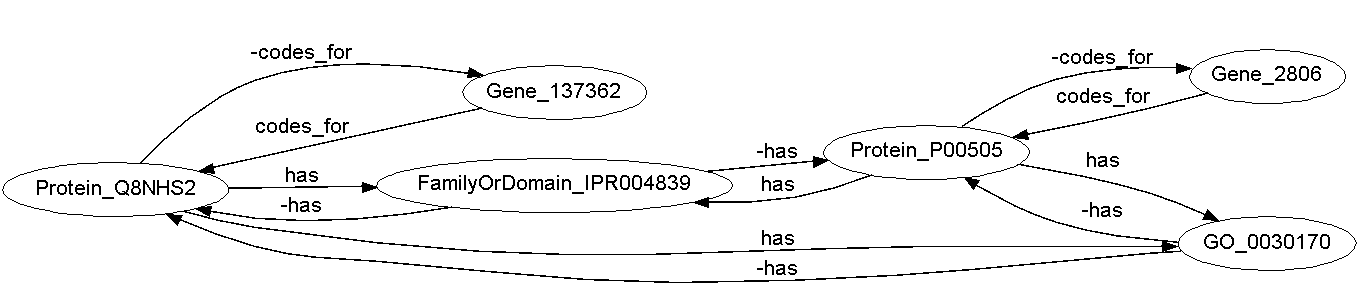
\includegraphics[width=16cm]{images/subgraph1.png}
\caption{Пример подграфа}
\label{subgraph}
\end{figure}

Существует большое количество биологических баз данных с открытым доступом, информация в которых может быть представлена как помеченный граф, в котором вершины соответствуют сущностям (протеины, гены, фенотипы), а рёбра отношениям между ними (взаимодействует, кодирует). Пути между вершинами позволяют найти новые связи в данных, либо показывают уже известные отношения. Подграф, построенный на всех найденных путях, более наглядно демонстрирует связи между вершинами. На рисунке \ref{subgraph} показан пример подграфа, построенного на путях между генами. 

Реальный набор биологических данных был собран из разных баз данных, находящихся в открытом доступе:  Entrez Gene (информация о генах), UniProt (протеины), Gene Ontology (биологические процессы), STRING (связи между протеинами), InterPro (семейства белков), KEGG (связи между генами), HomoloGene (группы гомологий генов). Данные были ограничены набором из пяти организмов: Homo sapiens, Rattus norvegicus, Mus musculus, D. melanogaster и C. elegans. Объединенные в один файл данные состоят из троек: субъект, отношение, объект. Такие тройки образуют помеченный ориентированный граф.
\subsection{Запросы}

\begin{figure}
$$
\begin{array}{crcl}
&\mbox{\texttt{ [<Start>] }} \\
&\mbox{\texttt{s}} &:& \mbox{\texttt{gene }} \\
&\mbox{\texttt{v}} &:& \mbox{\texttt{protein | gene | GO | PATHWAY | FAMDOM | HOMOLOGENE}} \\
&\mbox{\texttt{similar}} &:& \mbox{\texttt{CODESFOR v RCODESFOR | BELONGS v RBELONGS}} \\
&&&\mbox{\texttt{| HAS v RHAS | HOMOLOGTO v RHOMOLOGTO}} \\
&\mbox{\texttt{ps}} & :& \mbox{\texttt{ (PROTEIN similar) *[1..2]}} \\
&\mbox{\texttt{protein}} & :& \mbox{\texttt{ps PROTEIN | PROTEIN}} \\
&\mbox{\texttt{gs}} & :& \mbox{\texttt{(GENE similar) *[1..2]}} \\
&\mbox{\texttt{gene}} & :& \mbox{\texttt{gs GENE | GENE}} \\
\end{array}
$$
\caption{Грамматика на языке YARD}
\label{grammar}
\end{figure}

Все вершины в полученном графе имеют уникальную метку. Но для удобства будем различать их по типу: гены, фенотипы и т.д. Назовём две вершины в графе похожими, если они одного типа и имеют рёбра одного типа к похожим вершинам. Это определение рекурсивно. Таким образом, путь между похожими вершинами представляет собой палиндром, который нельзя задать с помощью регулярной грамматики. На рисунке \ref{grammar} показана КС-грамматика на языке YARD, которая определяет похожие гены.  
\subsection{Производительность}

\begin{figure}
\begin{center}
\begin{tikzpicture}
\begin{axis}[
    xlabel = {Количество рёбер, тыс},
    ylabel = {Время, с}
]
\addplot coordinates {
  (1.048,0.2) (2.334,0.68) (4.742,3.2) (7.046,8.7) (9.850,17.5) (12.398,30.7) (14.968,51.3) (17.432,84.2) (20.480,132)
};
\end{axis}
\end{tikzpicture}
\end{center}
\caption{Время работы алгоритма}
\label{time}
\end{figure}

Для оценки производительности была проведена серия экспериментов. Результаты приведены на графике, изображённом на рисунке \ref{time}. В статье \cite{subgraph} был проведён похожий эксперимент, но длины путей были ограничены от 4 до 8. В данной работе добиться такого ограничения не удалось, подграф строится по путям любой длины, поэтому нет возможности напрямую сравнить результаты.

\section{Заключение}
\begin{itemize}
    \item Реализована возможность поиска путей в графе с помеченными вершинами и рёбрами по заданной КС-грамматике.
    \item Реализовано получение подграфа с метками на вершинах и рёбрах.
    \item Проведена апробация алгоритма.
    
\end{itemize}
\setmonofont[Mapping=tex-text]{CMU Typewriter Text}
\bibliographystyle{ugost2008ls}
\bibliography{diploma.bib}
\end{document}
